\documentclass{zkdl-template}

\usepackage{opencolor}

\title{\huge\sffamily\bfseries ZKDL Lecture Notes}
\author{\Large\sffamily by \emph{Distributed Lab}}
\date{\sffamily \today \\ \vspace{1mm} Version 0.1}
%\titlepic{
\includegraphics[width=0.2\textwidth]{lectures/images/common/logo.png}}

\begin{document}

\pagestyle{fancy}

% --- Drawing a book cover ---

\colorlet{coverBackground}{oc-gray-0}
\colorlet{coverBoxBackground}{oc-gray-7}

\pagecolor{coverBackground}
\begin{tcolorbox}[
    standard jigsaw,
    colframe=coverBoxBackground, 
    colback=oc-gray-3,
    width=\textwidth, 
    halign=center, 
    valign=center, 
    %opacityback=0,
    arc=1em,
    shadow={4mm}{-3mm}{0mm}{black!30!white},
    enhanced,
    boxrule=5pt,
    rightrule=9pt,
    bottomrule=9pt]
    \maketitle
\end{tcolorbox}

% Include figure below

\vspace{1.5cm}
\begin{figure}[h]
    \centering
    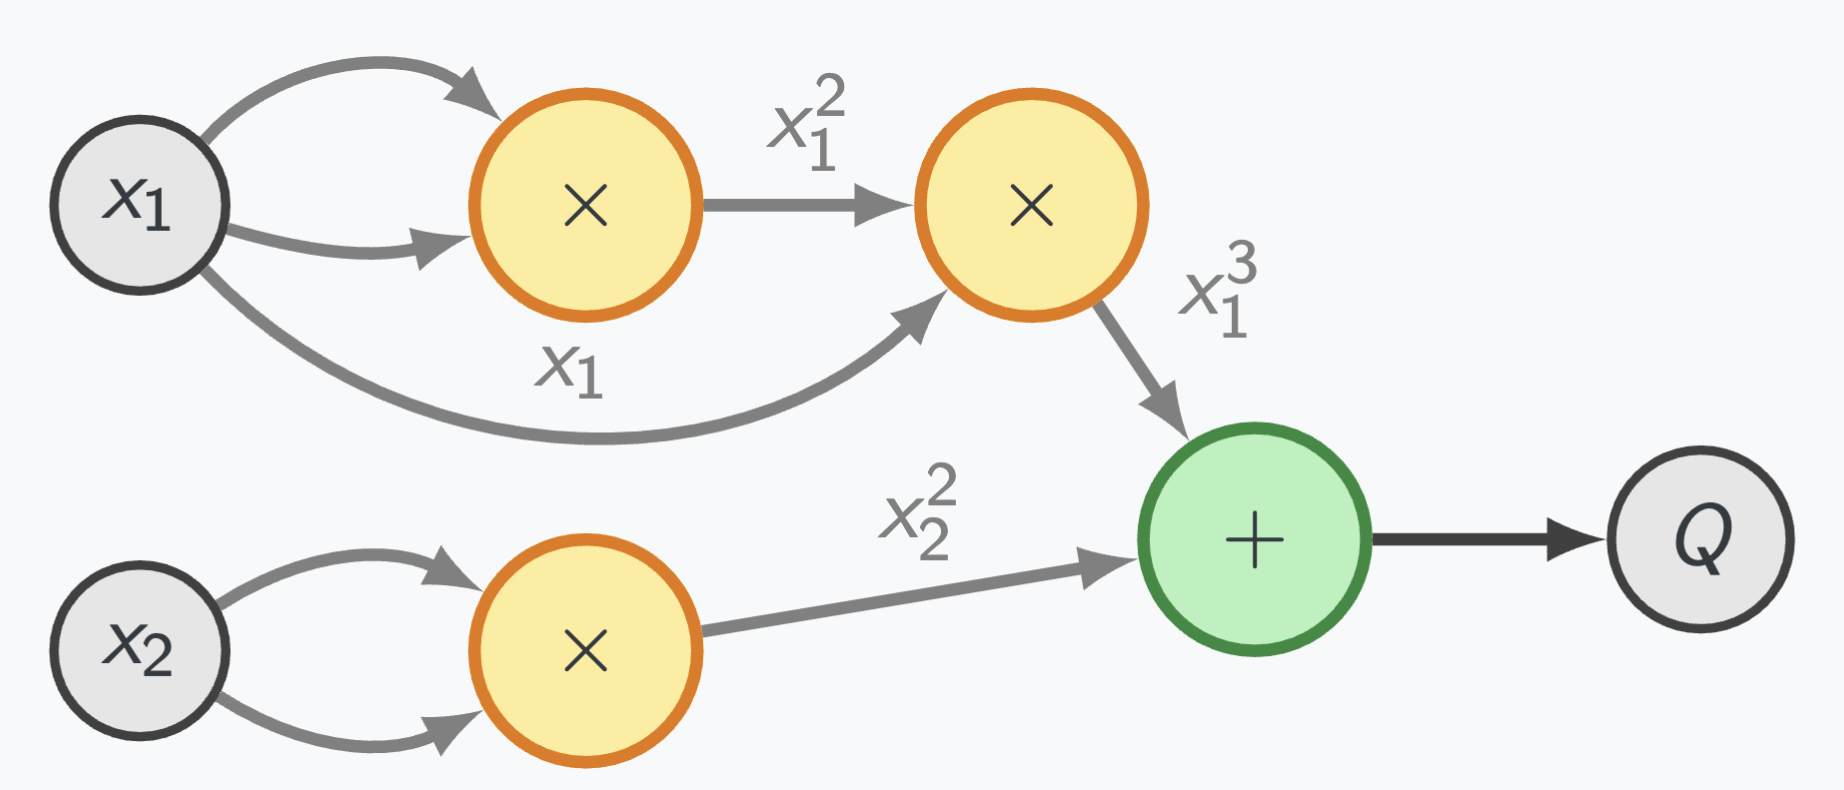
\includegraphics[width=0.8\textwidth]{lectures/images/cover-image-1.png}
\end{figure}

\newpage

\pagecolor{white}

\begin{abstract}
    Due to the rise of zero-knowledge technologies and their applications in
    various fields such as Blockchain or anonymous identity management, it is
    essential to develop a comprehensive understanding of the underlying
    mechanisms. However, the existing resources on the topic are either too
    high-level or too low-level, making it hard for regular practicing engineers
    to understand the practical implications of zero-knowledge protocols.

    This book aims to bridge this gap by providing a complete, practical guide
    to the state-of-the-art techniques in zero-knowledge cryptography, such as
    $\Sigma$-protocols, zk-SNARKs (Groth16 in particular), PlonK and more. We
    gathered all the necessary information in one place, and tried to make it
    easy to follow, with numerous examples and code snippets. We attach
    exercises to each chapter to help you understand the material better.
    Despite the book's practical focus, we preserve the mathematical rigor where
    suitable and necessary.
\end{abstract}

\newpage
% --- Table of Contents ---

\tableofcontents

\newpage

% --- Content ---

\section{Preface}

\subfile{preface}

\section{Group Theory and Polynomials}\label{section:math-crypto-1}

\subfile{lectures/1-math}

\section{Basics of Security Analysis}\label{section:math-crypto-2}

\subfile{lectures/2-math-and-crypto}

\section{Field Extensions and Elliptic Curves}

\subfile{lectures/3-ec}\label{section:field_extensions}

\section{Projective Coordinates and Pairing}

\subfile{lectures/4-pairing}

\section{Commitment Schemes}\label{section:commitments}

\subfile{lectures/5-commitments}

\section{Introduction to Zero-Knowledge Proofs}\label{section:intro-zk}

\subfile{lectures/6-intro-zk}

\section{Sigma Protocols}\label{section:sigma}

\subfile{lectures/7-sigma}

\section{Introduction to SNARKs. Arithmetic Circuits. R1CS}\label{section:r1cs}

\subfile{lectures/8-circuits}

\section{Quadratic Arithmetic Program. Probabilistically Checkable Proofs}\label{section:qap}

\subfile{lectures/9-qap-pcp}

\section{Pairing-based SNARKs. Pinocchio and Groth16}\label{section:groth16}

\subfile{lectures/10-groth}

\section{Circom}\label{section:circom}

\subfile{lectures/11-circom}

\section{PlonK}\label{section:plonk}

\subfile{lectures/12-plonk}

\end{document}
